
% {{{ preamble

%\documentclass[10pt,letterpaper]{article}
\documentclass{article}
%\documentclass[twocolumn]{article}
%\documentclass[12pt]{report}

\usepackage{url}
\usepackage{hyperref}
\usepackage{graphicx}
%\usepackage{multicol}
\usepackage{nonfloat}
\usepackage{amsmath}
\usepackage{mathtools}
\usepackage{parskip}
\usepackage{bloques}

\usepackage{tikz}
\usetikzlibrary{calc,arrows,positioning}
% control system tikz objects
\tikzset{shadow/.style={drop shadow={opacity=0.8},fill=white}}
\tikzset{sum/.style={circle,draw,very thick,shadow,minimum size=6mm}}
\tikzset{sumnp/.style={sum,
				label={{above left,xshift=1.0mm,yshift=-1.0mm}:$+$},
				label={{below left,xshift=1.0mm,yshift=1.0mm}:$-$}}}
\tikzset{sumxpxp/.style={sum,
				label={{above left,xshift=1.0mm,yshift=-1.0mm}:$+$},
				label={{above right,xshift=-1.0mm,yshift=-1.0mm}:$+$}}}
\tikzset{gain/.style={rectangle,draw,very thick,inner sep=2mm,shadow}}
%\newcommand{\nodesum}[2]{
%\node[sum]  (#1) [label={{above left,xshift=1.5mm,yshift=-1.5mm}:$+$},
%				  label={{below left,xshift=1.5mm,yshift=1.5mm}:$-$},#2] {};
%}

\usepackage{listings}
\lstset{numbers=left,
		language=Matlab,
		basicstyle=\footnotesize,
		captionpos=b,
		xleftmargin=0.3in}

\usepackage{sectsty}  % \sectionfont
\sectionfont{\normalsize}
\subsectionfont{\normalsize}

\usepackage{vmargin}  % make the margins a bit smaller
\setmarginsrb{1.0in}{1.0in}{1.0in}{1.0in}{0in}{0.25in}{0in}{0.20in}

\raggedright
%\setlength{\parindent}{0.2in}

%
% backend	: biber
% style		: numeric
% autocite	: footnote
% citestyle	: verbose-inote
% bibstyle	: authortitle, numeric
%
\usepackage[backend=biber,autocite=footnote,
			bibstyle=authortitle,citestyle=verbose-inote]{biblatex}

%\addbibresource{main.bib}
\addbibresource{control.bib}

% }}}

\begin{document}

% {{{ title page

\thispagestyle{empty}

\centerline{\Large \textbf{A Survey of Control Systems Applied to}}
\centerline{\Large \textbf{the Idle Control of an Automotive Engine}}
\vspace{0.1in}
\centerline{\normalsize {Jeremiah Mahler}}
\centerline{\small {\href{mailto:jmahler@mail.csuchico.edu}{jmahler@mail.csuchico.edu}} }
\vspace{0.1in}
\centerline{\normalsize {CSU Chico}}
%\centerline{\today}
%\vspace{0.1in}
\centerline{\small \today}
\vspace{0.2in}
\centerline{\LARGE \textbf{DRAFT}}
\vspace{0.2in}

% }}}

% {{{ abstract
%\pagebreak
%\thispagestyle{empty}
%\begin{abstract}
%\noindent

% TOOD

% What methods are used? PID, direct? ...

%\end{abstract}
% }}}

\section{Model}

The engine model used here is based work
by Butts and Sivashankar\autocite{532315} which is derived from
the work by Powell and Cook\autocite{4789342}.
The engine configuration is a modern 4.6L V-8.
To simplify analysis the linearized model is used as shown in
Figure \ref{fig:lem}.

\xdistance{1.8cm}
\ydistance{2.0cm}

\begin{figure}[hbp!]
\begin{center}
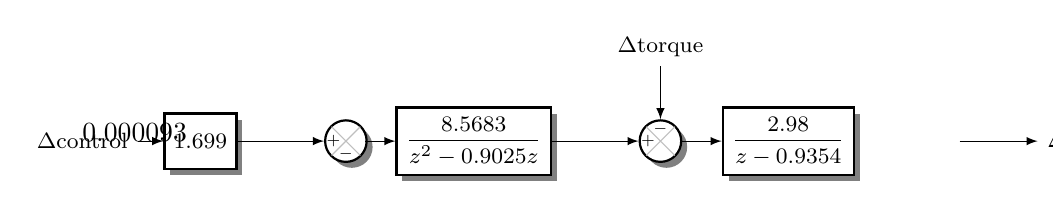
\begin{tikzpicture}
\bShadow
\bStart{$\Delta \text{control}$}
\bGain{$1.699$}
\bMinusF{S1}
\bGain{$\dfrac{8.5683}{z^2 - 0.9025 z}$}
\bMinusUp{$\Delta \text{torque}$}
\bGain{$\dfrac{2.98}{z - 0.9354}$}
\bGainFeedBack{$0.000093$}{S1}
\bEnd{$\Delta \text{rpm}$}
\end{tikzpicture}
\end{center}
\caption{Linear engine model.}\label{fig:lem}
\end{figure}

This model takes two inputs: a torque, and a idle control signal.
When the torque is greater than zero it will oppose the rotation of
the engine causing it to slow down.
The idle control signal is some fraction of unity.
This fraction corresponds to a pulse width modulated idle control valve
which is at a minimum near zero and at a maximum near unity.
Often the duty cycle range is in a range from 0\% to 100\% which
corresponds to 0 to 1 (unity).

This model has one complication that makes it difficult to use compared
to typical control systems.
All the inputs and outputs are specified as deltas ($\Delta$).
The torque input, for example, cannot be given as a constant ($T$) because this
actually means $\Delta T$

To overcome this complication a simple feedback controller can be used
as show in Figure \ref{fig:scont}.
And the open loop controller, with a fixed input duty cycle, is shown
in Figure \ref{fig:openloop}.
Notice that in this example the torque has transient characteristics and
varies over time.
The output of this system is show in Figure \ref{fig:olplot}.

\clearpage
\begin{figure}[!htbp]
\begin{center}

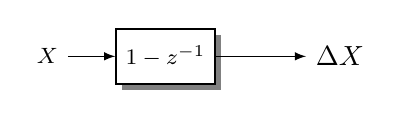
\begin{tikzpicture}
%\xdistance{1.2cm}
%\ydistance{1.5cm}
\bShadow
\bStart{$X$}
\bGain{$1 - z^{-1}$}
\bEnd{$\Delta X$}
\end{tikzpicture}

%\begin{tikzpicture}
%\xdistance{1.2cm}
%\ydistance{1.5cm}
%\bShadow
%\bStart{$X$}
%\bMinusF{S1}
%\bGain{$\Sigma$}
%\bFeedBack{}{S1}
%\bEnd{$\Delta X$}
%\end{tikzpicture}

\end{center}
\caption{$Z$ transform used to accumulate the input and convert
a steady state input to delta output.
See Appendix \ref{app:cdelta} for the derivation.}
\label{fig:scont}
\end{figure}

\begin{figure}[!htbp]
\begin{center}
\includegraphics[scale=0.5]{img/schematic-no_control-ed1}
\end{center}
\caption{Linear engine model with an open loop controller.
Inputs go through the simple controller to provide steps to the
engine model.
The output rpm, since it is in steps ($\Delta N$), is accumulated.}
\label{fig:openloop}
\end{figure}

\begin{figure}
\begin{center}
\includegraphics[scale=0.8]{img/linear_engine_model_no_control_plot}
\end{center}
\caption{Output of linear engine controller with a transient torque
input and a fixed input duty cycle.  Matlab source given in
Appendix \ref{app:olplot}}
\label{fig:olplot}
\end{figure}

% References
\clearpage
\printbibliography[heading=bibintoc]

\clearpage
\appendix

% {{{ Steady State to Delta $Z$ Transform Derivation
\section{Steady State to Delta $Z$ Transform Derivation}
\label{app:cdelta}

\begin{figure}
\begin{center}

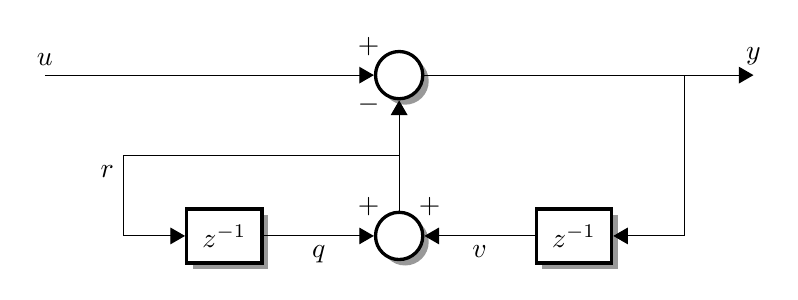
\begin{tikzpicture}[>=triangle 60,
	node distance=14mm, auto]
%	[inner sep=10mm, minimum size=6mm, node distance=20mm]

	\node[sumnp]  (sum1)	[] 					{};
	\node[sumxpxp] (sum2)	[below=of sum1] 	{};
	\node[gain] (gain1)		[right=of sum2]		{$z^{-1}$};
	\node[gain] (gain2)		[left=of sum2]		{$z^{-1}$};

	\draw [->] (sum2.north) -- 					(sum1.south);
	\draw [->] (gain1.west) -- node[below]{$v$} 	(sum2.east);
	\draw [->] (gain2.east) -- node[below]{$q$} 	(sum2.west);

	 \draw [->]
	 		($ (sum1.south) - (0,7mm) $)
			-- ++(-35mm,0) node[below left]{$r$} 
			|- (gain2.west);
	\draw [->]
			(-45mm,0) node[above] {$u$} to (sum1);
	\draw [->]
			(sum1) to (45mm,0) node[above] {$y$};
	\draw [->]
			($(sum1.east) + (33mm,0) $)
			|- (gain1);

\end{tikzpicture}

%\tikzstyle{block}=[draw,minimum size=2.4em]
%
%\tikzstyle{sum}=[draw,circle,minimum size=1.2em]
%
%%\tikzstyle{init} = [pin edge={to-,thin,black}]
%\begin{tikzpicture}[node distance=2.0cm,auto,>=latex']
%
%	% place all the block, points, relative to each other
%	\node [coordinate,node distance=2cm] (u) {u};
%	\node [block,right of=u] (k) {$K$};
%
%	\node [sum,right of=k] (s) {};
%
%	\node [coordinate,below of=s] (ds) {ds};
%	\node [block,right of=ds] (d) {$D(s)$};
%	\node [block,right of=s] (g) {$G(s)$};
%	\node [coordinate,right of=g] (gdy) {};
%	\node [coordinate,right of=gdy,node distance=2cm] (y) {y};
%	\node [coordinate,right of=d] (gd) {gd};
%
%	% add signs to sum
%	\node [left of=s,node distance=0cm,xshift=-3mm,yshift=3mm] {$+$};
%	\node [left of=s,node distance=0cm,xshift=-3mm,yshift=-4mm] {$-$};
%
%	% add labels to G(s) and D(s)
%	\node [right of=g,node distance=0cm,xshift=8mm,yshift=6mm] {$\dfrac{B}{A}$};
%	\node [right of=d,node distance=0cm,xshift=8mm,yshift=6mm] {$\dfrac{\beta}{\alpha}$};
%
%	% connect all the nodes and points
%	\path[->] (u) edge node {$u$} (k);
%	\path[->] (k) edge node {} (s);
%	\path[->] (ds) edge node {} (s);
%	\path[-]  (d) edge node {} (ds);
%	\path[->] (s) edge node {$\epsilon$} (g);
%	\path[-] (g) edge node {} (gdy);
%	\path[->] (gdy) edge node {$y$} (y);
%	\path[-] (gdy) edge node {} (gd);
%	\path[->] (gd) edge node {} (d);
%
%\end{tikzpicture}

\end{center}

\caption{System to accumulate values to convert a steady state
input to a delta output.}
\end{figure}

% }}}

\section{Linear Engine Model Plot Matlab Script}
\label{app:olplot}
\lstinputlisting[language=Matlab]{../matlab/linear_engine_model_plot.m}

\section{Linear Engine Model Initialization Matlab Script}
\lstinputlisting[language=Matlab]{../matlab/linear_engine_model_init.m}

\end{document}
